
\section{Long Term Modulation of Star Formation Rates}
\label{bursts:sec:oscillatory} 

\begin{figure*} % fig 8
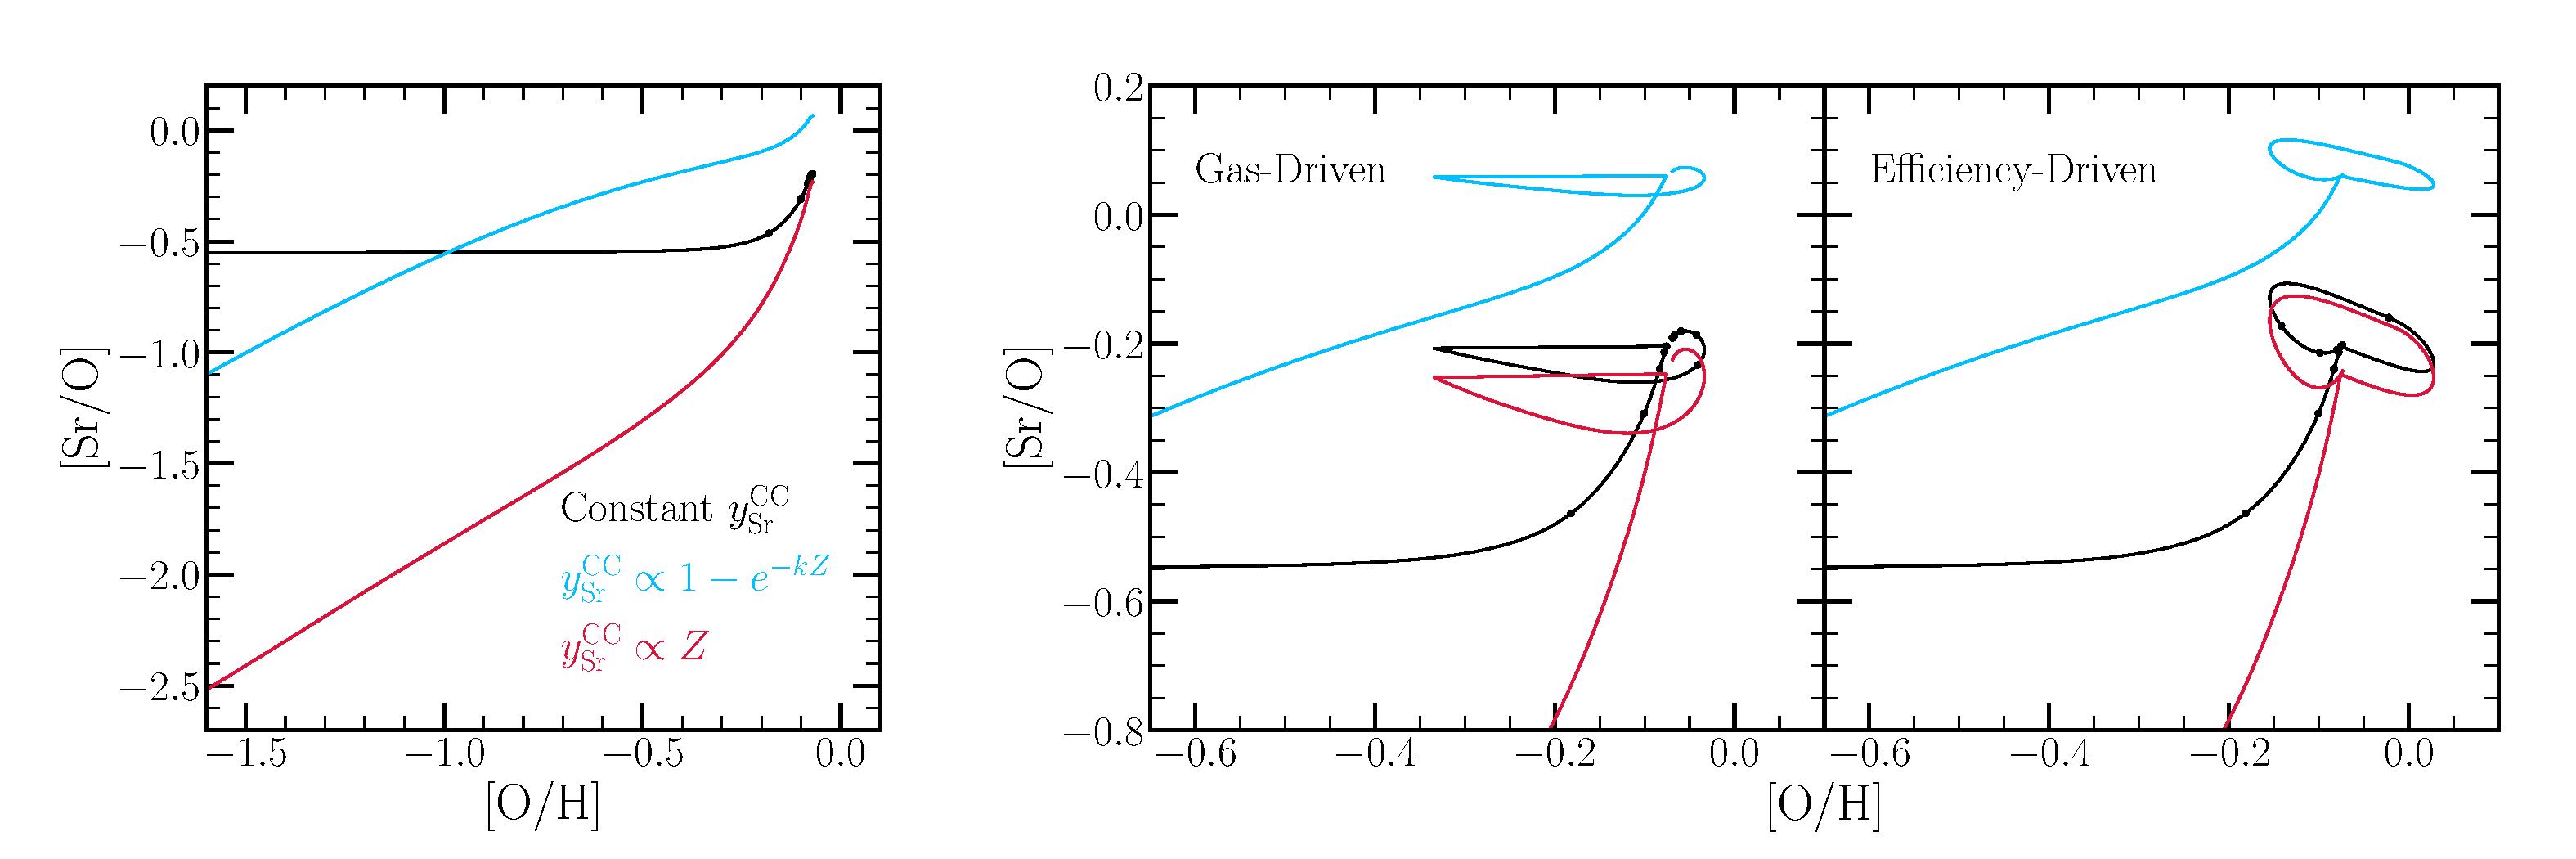
\includegraphics[scale = 0.32]{sro_bursts.pdf} 
\caption{
Evolutionary tracks in the [Sr/O]-[O/H] plane for our fiducial burstless 
model (left) and for our fiducial gas-driven (middle) or efficiency-driven 
(right) starburst models, for three models of the $y_\text{Sr}^\text{CC}$ yield 
as labeled. In contrast to Figs.~\ref{bursts:fig:sr_yields} and~\ref{bursts:fig:bursts_srfe}, 
these results are independent of SN Ia enrichment, simplifying interpretation. 
In the middle panels, tracks initially evolve to lower [O/H] because of gas 
dilution, while in the right panel they evolve to higher [O/H] because 
increased SFE reduces the gas supply. The [Sr/O] evolution is driven mainly by 
the metallicity dependence of the Sr yields. In all panels, 
points are plotted at 1-Gyr intervals on models shown in black. 
}
\label{bursts:fig:sro_bursts} 
\end{figure*} 

\begin{figure*} % fig 9
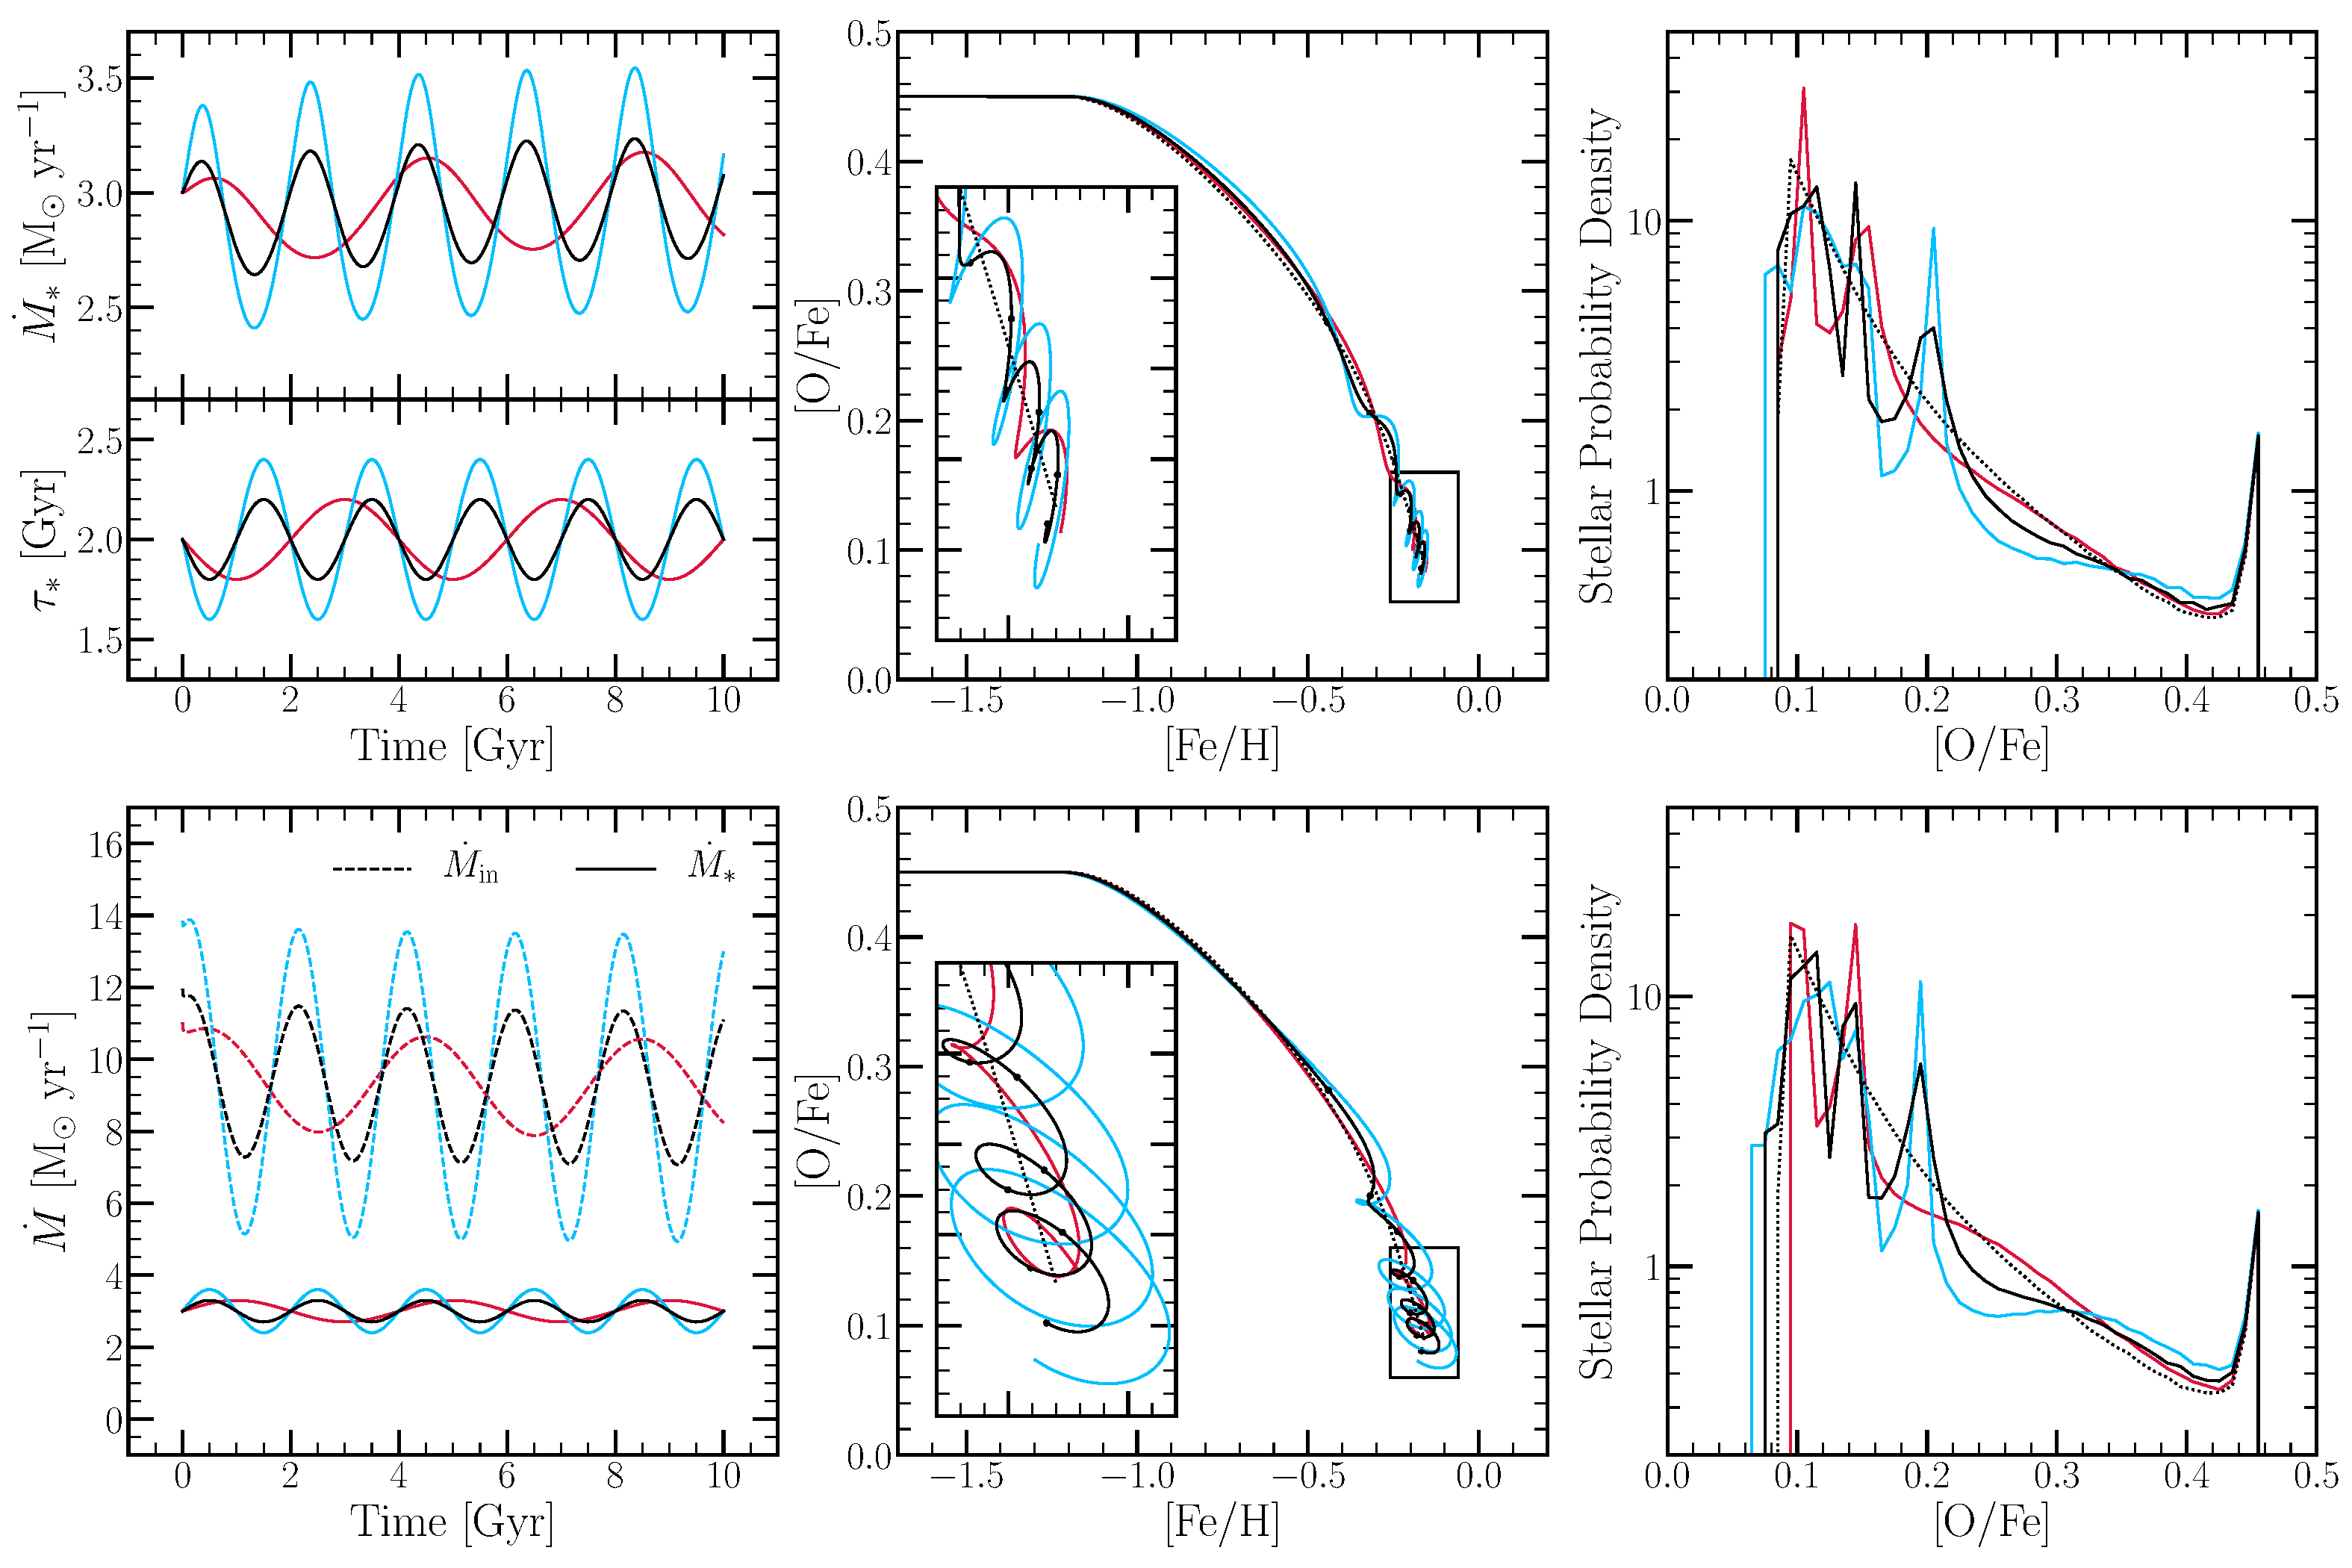
\includegraphics[scale = 0.32]{oscil.pdf} 
\caption{
Models with sinusoidal modulations of the SFR induced by modulations of the 
SFE timescale $\tau_*$ (top) or the gas infall rate $\dot{M}_\text{in}$ 
(bottom). Black curves represent a model with 10\% SFR modulations and a 2 Gyr 
period, while blue and red curves show the effect of doubling the amplitude or 
period of the modulation, respectively. In the middle and right panels, dotted 
black curves show results for our fiducial unperturbed model for comparison. 
In the middle panels, points are plotted at 1-Gyr intervals for the 10\% 
amplitude, 2-Gyr period model.
} 
\label{bursts:fig:oscil} 
\end{figure*} 

\begin{figure*} % fig 10 
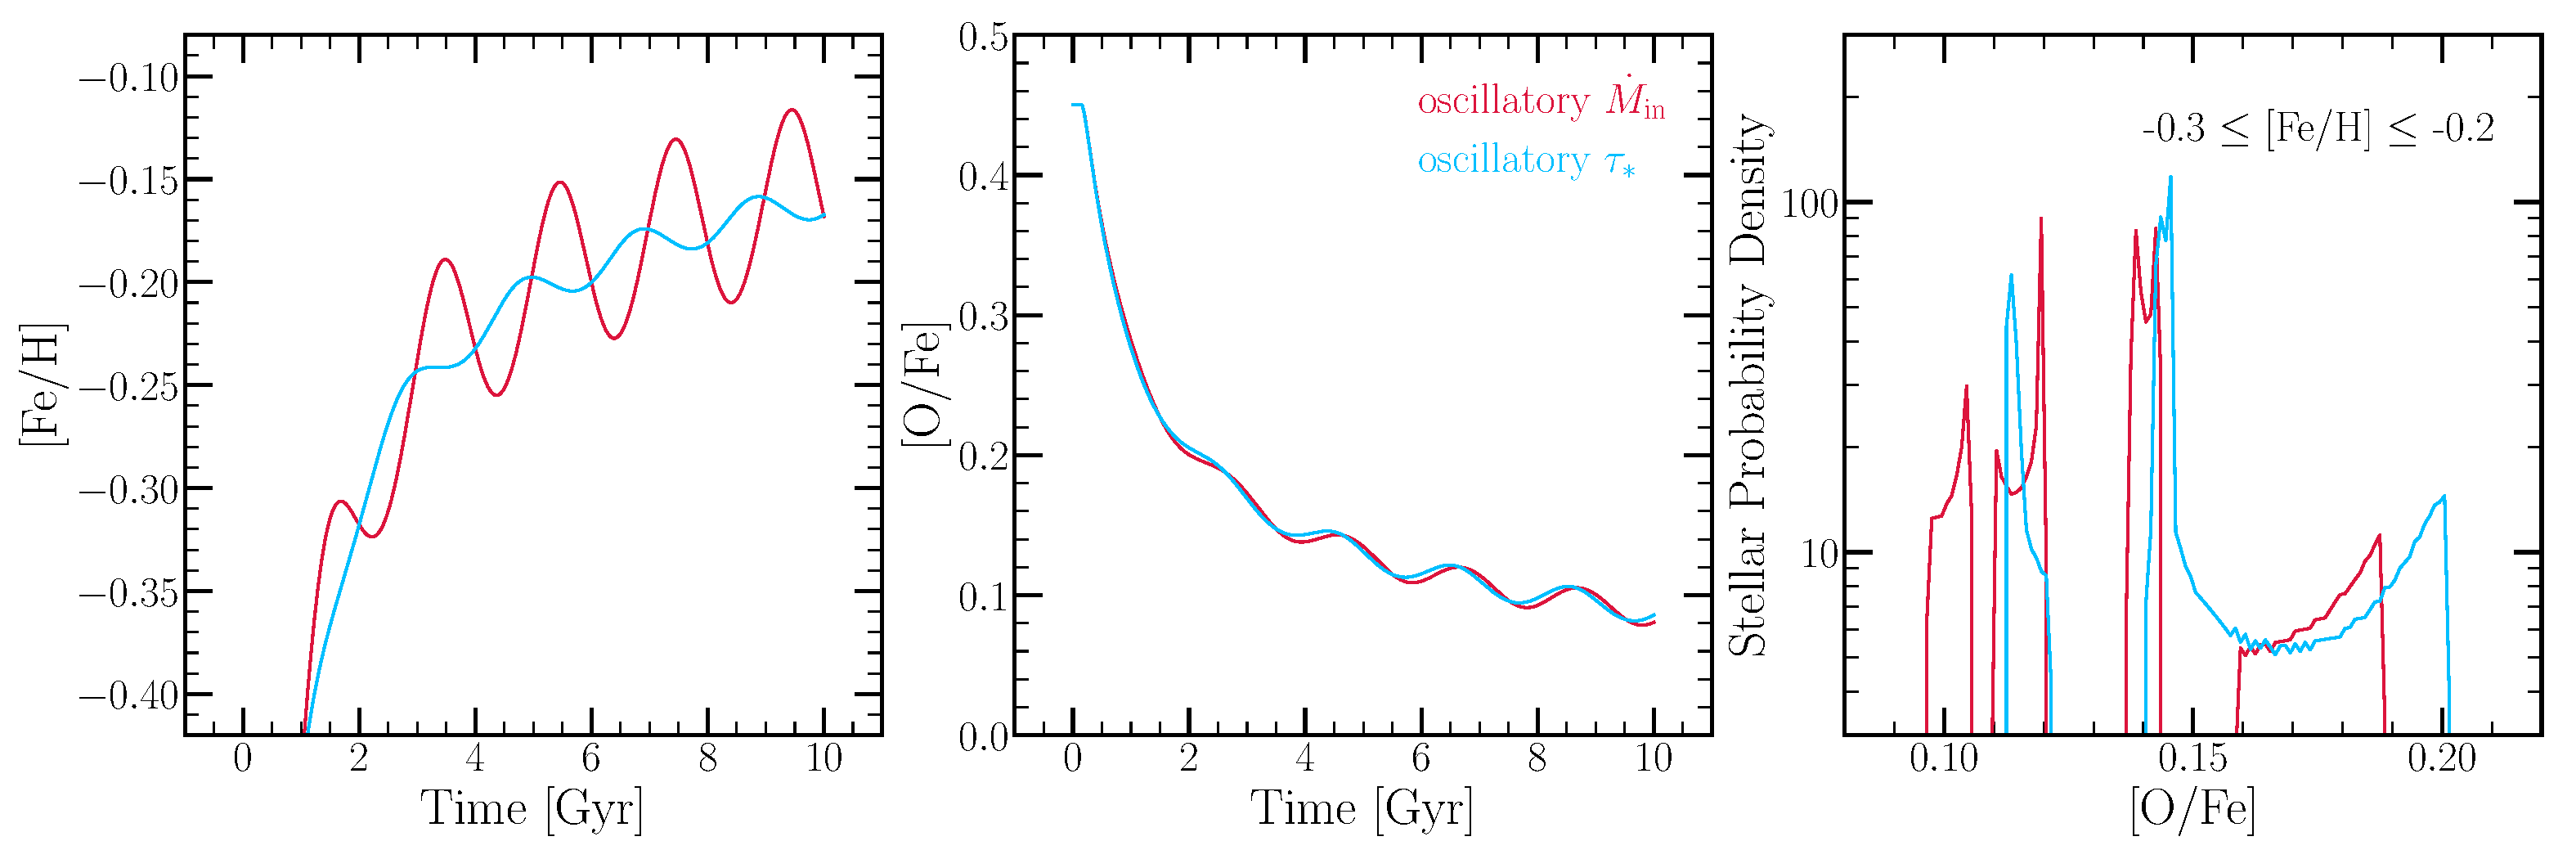
\includegraphics[scale = 0.32]{oscillations_v_time.pdf} 
\caption{
Time evolution of [Fe/H] (left) and [O/Fe] (middle) for the 20\% amplitude, 2 
Gyr models driven by $\tau_*$ modulations (red curves) or $\dot{M}_\text{in}$ 
modulations (blue curves). Oscillations of [Fe/H] are larger in the infall 
modulation model, but oscillations of [O/Fe] are similar in the two models. 
The right hand panel shows the [O/Fe] distributions for stars in the range 
-0.2$\leq$[Fe/H]$\leq$-0.3, demonstrating that at constant [Fe/H], the 
resultant [O/Fe] distribution is not a simple bimodal gaussian. 
} 
\label{bursts:fig:oscil_v_time} 
\end{figure*}

Bursts of star formation change the ratio of CCSNe to SNe Ia, producing loops 
in [O/Fe]-[Fe/H] trajectories and multiple peaks in [O/Fe] distributions. 
Slower, continuous variations of SFR also perturb the CCSN/SN Ia ratio in ways 
that can add complexity to these trajectories and distributions. From the 
standpoint of starbursts, such variations can be thought of as emulating a 
series of minor bursts throughout a galaxy's history, and are a possible 
source of scatter in [O/Fe] at fixed [Fe/H] in observed stellar populations. 
In the Milky Way disk,~\citet{BertranDeLis2016} estimate the intrinsic scatter 
in [O/Fe] as 0.03-0.04 dex in both the high-$\alpha$ (``chemical thick disk'') 
and low-$\alpha$ (``chemical thin disk'') stellar populations. 
\par
Fig.~\ref{bursts:fig:oscil} shows evolutionary tracks and [O/Fe] distributions for 
models with sinusoidal perturbations in SFR relative to a constant SFR model. 
In the upper panels, we create the SFR variations by modulating the SFE 
timescale $\tau_*$ about its baseline value of 2 Gyr. The black curve shows a 
model in which the amplitude of modulation is 10\% (i.e. 0.2 Gyr) and the 
period of modulation is 2 Gyr. Blue and red curves show models with a 20\% 
amplitude and a 4 Gyr period, respectively. The gas infall rate 
$\dot{M}_\text{in}$ and the outflow efficiency $\eta$ are held constant at 
their fiducial values. 
\par 
As one might expect from our efficiency-driven starburst models, each 
oscillation in $\tau_*$ induces a low amplitude loop in the [O/Fe]-[Fe/H] 
trajectory. For a 2 Gyr period, the first minimum in SFR occurs when [Fe/H] 
$\approx$ -0.45, and at lower metallicties the trjectory is only slightly 
different from that of an unperturbed model. At higher metallicities, there 
is a local maximum in [O/Fe] associated with each maximum in SFR, as one can 
see from the inset in the middle panel. The resulting [O/Fe] distributions 
have multiple peaks and troughs associated with flat and steep portions of the 
[O/Fe] trajectories, though these peaks can merge with each other into 
broader features. The peaks are sharper for higher amplitude modulations as 
expected. For the 10\% modulation, 2 Gyr period model there are three distinct 
peaks at [O/Fe] $\approx$ +0.11, +0.15, and +0.20, respectively, while the 
model with 4 Gyr period produces two distinct peaks at [O/Fe] $\approx$ +0.10 
and +0.15. 
\par 
The lower panels of Fig.~\ref{bursts:fig:oscil} show models in which we modulate 
the gas infall rate $\dot{M}_\text{in}$ while keeping $\tau_*$ and $\eta$ 
fixed. For these models we have chosen to modulate the \textit{star formation 
rate} $\dot{M}_*$ by 10\% or 20\% with a 2 or 4 Gyr period (solid curves in 
left panel). \texttt{VICE} automatically solves for the required modulations in 
$\dot{M}_\text{in}$ (dashed curves), which have the same period as the SFR 
modulations but a different phase and larger fractional amplitude. These gas 
supply modulations produce loops in [O/Fe] trajectories that resemble those of 
our infall-driven burst models. In particular, trajectories first move to lower 
[Fe/H] because of dilution, then to higher [O/Fe] and [Fe/H] because of 
subsequent star formation. The resulting [O/Fe] distributions show a multi-peak 
structure like that in the $\tau_*$-modulation models, with peaks at similar 
locations. 
\par 
Fig.~\ref{bursts:fig:oscil} shows that moderate amplitude fluctuations (10-20\%) of 
the SFR can produce a spread of [O/Fe] values at fixed [Fe/H], at 
the~$\sim$0.05-dex level. For $\tau_*$ modulations, this scatter appears 
mainly in the [O/Fe] dimension while for $\dot{M}_\text{in}$ modulations it 
appears in both the [O/Fe] and [Fe/H] dimensions, but the impact on the [O/Fe] 
distributions is similar. This is demonstrated further in the left and middle 
panels of Fig.~\ref{bursts:fig:oscil_v_time}, which compares the 20\% amplitude, 2-Gyr 
period models of the two modes of oscillations. The middle panel shows that 
both modes of oscillation produce strikingly similar evolution of the ISM 
[O/Fe] with time, but the oscillatory $\dot{M}_\text{in}$ model predicts much 
stronger oscillations in [Fe/H]. 
These results are in good agreement with the episodic SFH model for the 
Milky Way bulge in~\citet{Matteucci2019}, which shows qualitatively similar 
behavior in the [$\alpha$/Fe]-[Fe/H] plane. 
\par 
We also demonstrate in Fig.~\ref{bursts:fig:oscil_v_time} that these moderate 
variations do not produce a bimodal distribution in [O/Fe] at fixed [Fe/H] 
as observed in the Milky Way; a more dramatic departure from this class of 
models is required. The right panel shows the normalized stellar MDFs in [O/Fe] 
only considering stars with -0.3 $\leq$ [Fe/H] $\leq$ -0.2, and although these 
display complex structure, neither model reproduces the [O/Fe] distribution 
found by, e.g.,~\citet{BertranDeLis2016}, which is well described by two 
Gaussians separated by~$\sim$0.15 dex. It is also notable that these SFR 
modulations only induce scatter in [O/Fe] at locations well beyond the knee 
of the [O/Fe]-[Fe/H] track. In part this is because our chosen parameters 
predict models which evolve past the knee quickly, before a full cycle of the 
SFR modulation. However, enrichment near the [O/Fe] plateau is dominated by 
CCSN in any case, so fluctuations in the SFR that change the CCSN rate have 
little leverage on [O/Fe]. Explaining intrinsic scatter in [O/Fe] (or ratios 
for other $\alpha$-elements) near the plateau of the high-$\alpha$ sequence 
requires a different mechanism, such as incomplete mixing of CCSN ejecta that 
individually have varying [O/Fe] ratios. 

